Pierwszym krokiem jest opisanie w kilku słowach funkcjonalności.
\begin{code}
	\lstinputlisting[linerange={0-4}]{../meetspace/features/events.feature}
\end{code}\\

Następnie tworzymy scenariusz, w którym krok po kroku będziemy wykonywać czynności aż otrzymamy efekt końcowy. W tym przypadku będzie to wyświetlenie nowo dodanego wydarzenia.

Słowem kluczowym \textbf{,,Scenario''} nadajemy tytuł nowego scenariusza. Jest to o~ tyle pomocne, że w momencie uruchomienia testów, widać który scenariusz jest w tej chwili testowany.

\begin{code}
	\lstinputlisting[linerange={10-10}, firstnumber=5]{../meetspace/features/events.feature}
\end{code}\\

Słowem \textbf{,,Given''} definiujemy stan początkowy aplikacji, czyli miejsce, w którym będziemy zaczynać wykonywanie konkretnych czynności. W tym przypadku jest to strona główna oraz proces logowania. Zalogowanie się do aplikacji jest istotnym elementem, ponieważ, bez tego nie będziemy w stanie dodać żadnego nowego wydarzenia.

\begin{code}
	\lstinputlisting[linerange={7-8}, firstnumber=6]{../meetspace/features/events.feature}
\end{code}\\

Następnie użytkownik aby utworzyć wydarzenie musi kliknąć przycisk ,,Utwórz wydarzenie'', oraz wypełnić formularz odpowiednimi danymi: nazwa, data, data zakończenia, czas rozpoczęcia, plan i logo.

\begin{code}
	\lstinputlisting[linerange={11-17}, firstnumber=8]{../meetspace/features/events.feature}
\end{code}\\

Po słowie \textbf{,,Then''} definiujemy nasze oczekiwania. W tym przypadku chcemy zobaczyć nowo dodane wydarzenie wraz z jego wszystkimi właściwościami. Słowa \textbf{,,And''} używamy jeśli chcemy rozwinąć listę wykonywanych kroków lub listę oczekiwań.

\begin{code}
	\lstinputlisting[linerange={19-24}, firstnumber=15]{../meetspace/features/events.feature}
\end{code}\\

W ten sposób mamy opisaną, za pomocą testu integracyjnego, całą ścieżkę, którą musi przejść użytkownik, aby stworzyć nowe wydarzenie.

W przypadku gdy chcemy przetestować edytowanie istniejącego już wpisu, nie musimy przechodzić procesu tworzenia od początku. Wystarczy, że na wstępie stworzymy już gotowe wydarzenie, które w następnych krokach będzie modyfikowane.

\begin{code}
	\lstinputlisting[linerange={26-29}, firstnumber=1]{../meetspace/features/events.feature}
\end{code}\\

W tej chwili w bazie testowej mamy zapisany jeden rekord. Dane z jakimi tworzone jest wydarzenie nie mają w tym momencie najmniejszego znaczenia, nie to jest tutaj testowane. Równie dobrze można by wpisać dowolny ciąg znaków, ale kierujemy się dobrą praktyką programistyczną i staramy się pisać zrozumiały kod.

Aby móc edytować jakikolwiek wpis, musimy wejść na jego stronę i kliknąć odpowiedni przycisk, bądź link, żeby przejść do strony z formularzem.

\begin{code}
	\lstinputlisting[linerange={30-31}, firstnumber=5]{../meetspace/features/events.feature}
\end{code}\\

Zmieniamy wpisane wartości na ,,Party'' oraz ,,15:00 Start'' oraz ustawiamy nowe logo.

\begin{code}
	\lstinputlisting[linerange={32-35}, firstnumber=7]{../meetspace/features/events.feature}
\end{code}\\

I na koniec oczekujemy, że wprowadzone przed chwilą zmiany zobaczymy na stronie wydarzenia.

\begin{code}
	\lstinputlisting[linerange={38-39}, firstnumber=6]{../meetspace/features/events.feature}
\end{code}

Można łatwo zauważyć, że część kroków powtarza się w pierwszym jak i w drugim scenariuszu. Jest to nic innego jak zastosowanie metody DRY\footnote{Don't repeat yourself - Nie powtarzaj się}. Dzięki temu nowe testy powstają coraz szybciej i sprawniej.

W całym projekcie testów integracyjnych jest znacznie więcej. Oprócz wyżej pokazanego przykładu, testujemy również logowanie do aplikacji poprzez portal Facebook, wyszukiwanie wydarzeń, czy zapisywanie się na newsletter.

Rysunek nr \ref{fig:rspec} przedstawia rezultat wszystkich testów integracyjnych. W sumie 12 scenariuszy i 78 kroków, wszystkie spełnione pomyślnie.

\begin{figure}[h]
  \centering
  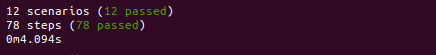
\includegraphics[scale=0.8]{images/bdd_result.png}
  \caption{Wyniki końcowe testów integracyjnych.}
  \label{fig:rspec}
\end{figure}

\newpage
